\documentclass[12pt]{article}
\usepackage[utf8]{inputenc}

\usepackage{amsthm}
\theoremstyle{plain}

\usepackage{amsmath}
\usepackage[utf8]{inputenc}
\usepackage[english]{babel}
\usepackage[citestyle=alphabetic,minalphanames=5]{biblatex}
\usepackage{hyperref}
\usepackage[margin=1in]{geometry}
\usepackage{graphicx}
\usepackage{float}

\setlength{\parindent}{0pt}
\setlength{\parskip}{10pt}

\newtheorem{proposition}{Proposition}[section]
\newtheorem{remark}[proposition]{Remark}

\addbibresource{master.bib}

\begin{document}

\section{Expansion of the solution of Volterra integral equation with inverse Mellin transform}

\subsection{Derivation of the asymptotic}

The log-mgf in the Rough Heston model is given by

\begin{equation} \label{logmgf}
m(s, t) = \log \mathbb{E}\left[e^{s X_{t}}\right]=\bar{v} \lambda I^{1} \psi(s, t)+v_{0} I^{1-\alpha} \psi(s, t)
\end{equation}

where $\psi$ satisfies the fractional Riccati equation

$$
\begin{aligned}
D^\alpha\psi(s,t) &= R(s, \psi(s, t)), \qquad \psi(0, \cdot) = 0
\end{aligned}
$$

and 

$$
R(s, w) = \frac{1}{2}\left(s^{2}-s\right)+(\rho \xi s - \lambda) w+\frac{1}{2} \xi ^{2} w^{2}.
$$

It is known from \cite{GGP18} that for a particular choice of parameters the solution explodes in finite time (cases A and B). We proceed with this assumption.

Fractional Riccati equations like above are in one-to-one correspondence with Volterra integral equations, hence we can rewrite the above as

\begin{equation} \label{eq: original volterra equation}
\psi(s,t) = \frac{1}{\Gamma(\alpha)} \int _0^t (t-\tau)^{\alpha-1} R(s, \psi(s, \tau)) d\tau.
\end{equation}

Now we want to reparametrize the equation. Define $\eta _0 := \frac{1}{T^*}$ and define

\begin{equation} \label{mellin w}
w(\eta) := \psi\left(s, T^* - \frac{1}{\eta + \eta_0}\right)
\end{equation}

We now fix $s$, plug in the definition of $\eta$ and perform a substitution $\tau = T^* - \frac{1}{\zeta + \eta _0}$ to reformulate \eqref{eq: original volterra equation} in terms of $w(\eta)$ as

\begin{equation} \label{eq: reformulated volterra equation}
w(\eta) = \int _0 ^\eta k\{(\eta - \zeta)[(\eta + \eta_0)(\zeta + \eta_0)]^{-1}\} \cdot (\zeta + \eta _0) ^{-2} R(s, w(\zeta)) d\zeta
\end{equation}

where $k(\eta) := \frac{1}{\Gamma(\alpha)} \eta^{\alpha - 1}$ is the kernel of the integral.

We set $\zeta = \eta \omega$ to remove $\eta$ from the integral bounds and obtain

$$
\begin{aligned}
w(\eta) &= \int_0^1 k\{\eta(1-\omega)[(\eta\omega +\eta_0)(\omega + \eta_0)]^{-1}\} \cdot (\eta \omega + \eta _0) ^{-2} R(s, w(\eta \omega)) d(\eta\omega)\\[10pt]
&= \eta \cdot \left(\frac{\eta}{\eta+\eta_0}\right)^{\alpha-1} \int^\infty_0 K(\omega)F(\eta\omega)d\omega\\[10pt]
&\sim \eta \cdot \int^\infty_0 K(\omega)F(\eta\omega)d\omega
\end{aligned}
$$

where 

$$
K(\omega) = \frac{1}{\Gamma(\alpha)}(1-\omega)^{\alpha-1}\theta(1-\omega), \qquad F(\eta\omega) = (\eta\omega + \eta_0)^{-1-\alpha} R(s, w(\eta \omega)).
$$

The integral looks now like a Mellin convolution, and this reformulation allows us to utilize Mellin transform technique described in \cite{BH75} and \cite{BBO00}.

We now employ the Parseval formula for Mellin transform for $w(\eta) = \eta I(\eta)$ and obtain

$$
w(\eta) \sim \frac{\eta}{2 \pi i} \int_{c-i \infty}^{c+i \infty} \mathrm{M}[K(\omega) ; 1-z] \mathrm{M}[F(\eta \omega) ; z] d z
$$

where the vertical path of integration lies within the fundamental strip of both Mellin transforms.

\paragraph{Mellin transform of the kernel}

Mellin transform of the kernel is

\begin{equation}\label{eq: mellin transform of kernel}
\mathrm{M}[K(\omega) ; 1-z]=\frac{1}{\Gamma(\alpha)} \int_{0}^{1} \omega^{z-1}(1-\omega)^{\alpha-1} d \omega=\frac{\Gamma(1-z)}{\Gamma(1+\alpha-z)}.
\end{equation}

$\Gamma(1-z)$ has poles at $1, 2, 3, 4, \dots$ with residues $\frac{(-1)^{n}}{n !}$, hence $\frac{\Gamma(1-z)}{\Gamma(1+\alpha-z)}$ is holomorphic for $z < 1$. We obtain the asymptotic 

\begin{equation} \label{eq: ultimate mellin}
w(\eta) \sim \frac{\eta}{2 \pi i} \int_{c-i \infty}^{c+i \infty} \frac{\Gamma(1-z)}{\Gamma(1+\alpha-z)} M[F(\eta \omega) ; z] d z, \qquad \eta \rightarrow \infty.
\end{equation}

\paragraph{Mellin transform of the non-linearity}

We now employ the ansatz

\begin{equation} \label{eq: mellin ansatz}
w(\eta) = \sum_{k=1}^{-\infty} d_k \eta^{\alpha k} = d_1 \eta^\alpha + d_0 + d_{-1} \eta ^ {-\alpha} + \dots
\end{equation}

which yields

$$
\begin{aligned}
F(\eta\omega) &= (\eta\omega)^{-1-\alpha}\left(\frac 12 \xi^2 d_1^2  (\eta\omega)^{2\alpha} + (\xi^2 d_0d_1 + (\rho\xi s - \lambda) d_1)(\eta\omega)^{\alpha} + O(1)\right)\\
&= \frac 12 \xi^2 d_1^2  (\eta\omega)^{-1+\alpha} + (\xi^2 d_0d_1 + (\rho\xi s - \lambda) d_1)(\eta\omega)^{-1} + O((\eta\omega)^{-1-\alpha}).
\end{aligned}
$$

Due to linearity of the Mellin transform we can now calculate the transform termwise. The first term can be written as

$$
\begin{aligned}
M\left[\frac{1}{2} \xi^{2} d_{1}^{2} (\eta\omega)^{-1+\alpha}; z\right] &= \frac{1}{2} \xi^{2} d_{1}^{2} \int _0 ^\infty (\eta \omega) ^ {-(1-\alpha)} \omega ^{z-1} d\omega \\
&= \frac{1}{2} \xi^{2} d_{1}^{2} \eta ^{-(1-\alpha)}\int _0 ^\infty \omega ^ {-(1-\alpha)} \omega ^{z-1} d\omega \\
&= \frac{1}{2} \xi^{2} d_{1}^{2} \eta ^{-(1-\alpha)} \left. \frac{\omega^{z-(1-\alpha)}}{z-(1-\alpha)} \right|^\infty _0 \\
&= \frac{1}{2} \xi^{2} d_{1}^{2} \frac{\eta ^{-z}}{z-(1-\alpha)}
\end{aligned}
$$

where we restricted $z<1-\alpha$, thus $\lim _{\omega \rightarrow \infty} \omega ^{z-(1-\alpha)} = 0$ and behavior of $\omega\rightarrow 0$ and $\eta \rightarrow \infty$ cancels out.

Similarly for the second term we get

$$
\begin{aligned}
M\left[(\xi^2 d_0d_1 + (\rho\xi s - \lambda) d_1) (\eta\omega)^{-1}; z\right] &= (\xi^2 d_0d_1 + (\rho\xi s - \lambda) d_1) \int _0 ^\infty (\eta\omega)^{-1} \omega ^{z-1} d\omega \\
&= (\xi^2 d_0d_1 + (\rho\xi s - \lambda) d_1) \eta ^{-1}\int _0 ^\infty \omega ^ {-1} \omega ^{z-1} d\omega \\
&= (\xi^2 d_0d_1 + (\rho\xi s - \lambda) d_1) \eta ^{-1} \left. \frac{\omega^{z-1}}{z-1} \right|^\infty _0 \\
&= (\xi^2 d_0d_1 + (\rho\xi s - \lambda) d_1) \frac{\eta ^{-z}}{z-1}
\end{aligned}
$$

where we again restricted $z<1$.

Hence we see that powers in the expansion of $F(\eta)$ correspond to the poles of the Mellin transform. $M[F; z]$ has poles at $1-\alpha, 1, 1+\alpha, 1+2\alpha, \dots$ with residues resulting from the coefficients of \eqref{eq: mellin ansatz} and model parameters. We write

$$
\eta^z M[F(\eta\omega); z] = \frac{\frac 12 \xi^2 d_1^2}{z - (1-\alpha)} + \frac{\xi^2 d_0d_1 + (\rho\xi u - \lambda) d_1}{z - 1} + \dots
$$

\paragraph{Shifting the contour and coefficient matching}

Note that $M[F(\eta\tau);z]$ is holomorphic $z<1-\alpha$, and since Mellin transform of the kernel from \eqref{eq: mellin transform of kernel} is holomorphic for $z<1$, the entire integrand is holomorphic for $z < 1-\alpha$. Hence the contour in the integral \eqref{eq: ultimate mellin} should lie within $\Re (z) < 1 - \alpha$. Note that both factors have a simple pole at $z=1$.

The original contour lies to the left of all the poles listed. Shifting the contour to the right allows us to collect the expansion terms, provided that the integrand is vanishing at $z \rightarrow \pm i\infty$.

We recall Cauchy integral formula

$$
f^{(n)}(a)=\frac{n !}{2 \pi i} \oint_{\gamma} \frac{f(z)}{(z-a)^{n+1}} d z.
$$

For $\gamma$ enclosing $z=1-\alpha$ we get

$$
\begin{array}{l}
\frac{\eta}{2 \pi i} \int_\gamma \frac{\Gamma(1-z)}{\Gamma(1+\alpha-z)} M[F(\eta \tau) ; z] d z \\ [10pt]
= \eta \cdot \frac{\Gamma(\alpha)}{\Gamma(2\alpha)} \cdot \text{Res} (M[F(\eta\tau); z], 1-\alpha) \\ [10pt]
= \eta ^\alpha \cdot \frac{\frac 12 \xi^2 \Gamma(\alpha)}{\Gamma(2\alpha)}   d_1 ^2.
\end{array}
$$

For $\gamma$ enclosing $z=1$ we have a double pole and therefore

$$
\begin{array}{l}
\frac{\eta}{2 \pi i} \int_\gamma \frac{\Gamma(1-z)}{\Gamma(1+\alpha-z)} M[F(\eta \tau) ; z] d z \\ [10pt]
= \eta \cdot \text{Res}(\Gamma(1-z), 1) \cdot \text{Res}(M[F(\eta \tau); z], 1) \cdot \left. [f'(z)] \right| _{z = 1, f(z) = \frac{\eta^{-z}}{\Gamma(1+\alpha-z)}} \\ [10pt]
= (\xi^{2} d_{0} d_{1}+(\rho \xi s-\lambda) d_{1}) \frac{-\log (\eta) \Gamma(\alpha) + \Gamma'(\alpha)}{\Gamma(\alpha)^2}.
\end{array}
$$

Matching the coefficients from our ansatz \eqref{eq: mellin ansatz} leads to

$$
\begin{aligned}
w(\eta) &= \frac{\Gamma(2\alpha)}{\frac 12 \xi^2 \Gamma(\alpha)} \eta^\alpha + \frac{ \rho\xi s - \lambda}{ \frac{\frac12 \xi^ 2 \Gamma(\alpha)^3}{\Gamma(2\alpha) \Gamma'(\alpha)} - \xi^2} + O(\eta^{-\alpha})\\[10pt]
&=: \Theta_0 \eta^{\alpha} + \Theta_1 + O(\eta^{-\alpha}).
\end{aligned}
$$

\subsection{Numerical experiment}

Here we take a look at the numerical solution of the fractional Riccati equation as suggested in \cite{ER16} and compare it to the asymptotic from the previous section. Note that both log-mgf (and its numerical solution) and approximation only depend on model parameters $\alpha$, $\rho$, $\xi$ and $\lambda$ and the moment $s$ (i.e. they do not depend on base and mean reversion level of the variance).

\begin{figure}[H]
    \centering
    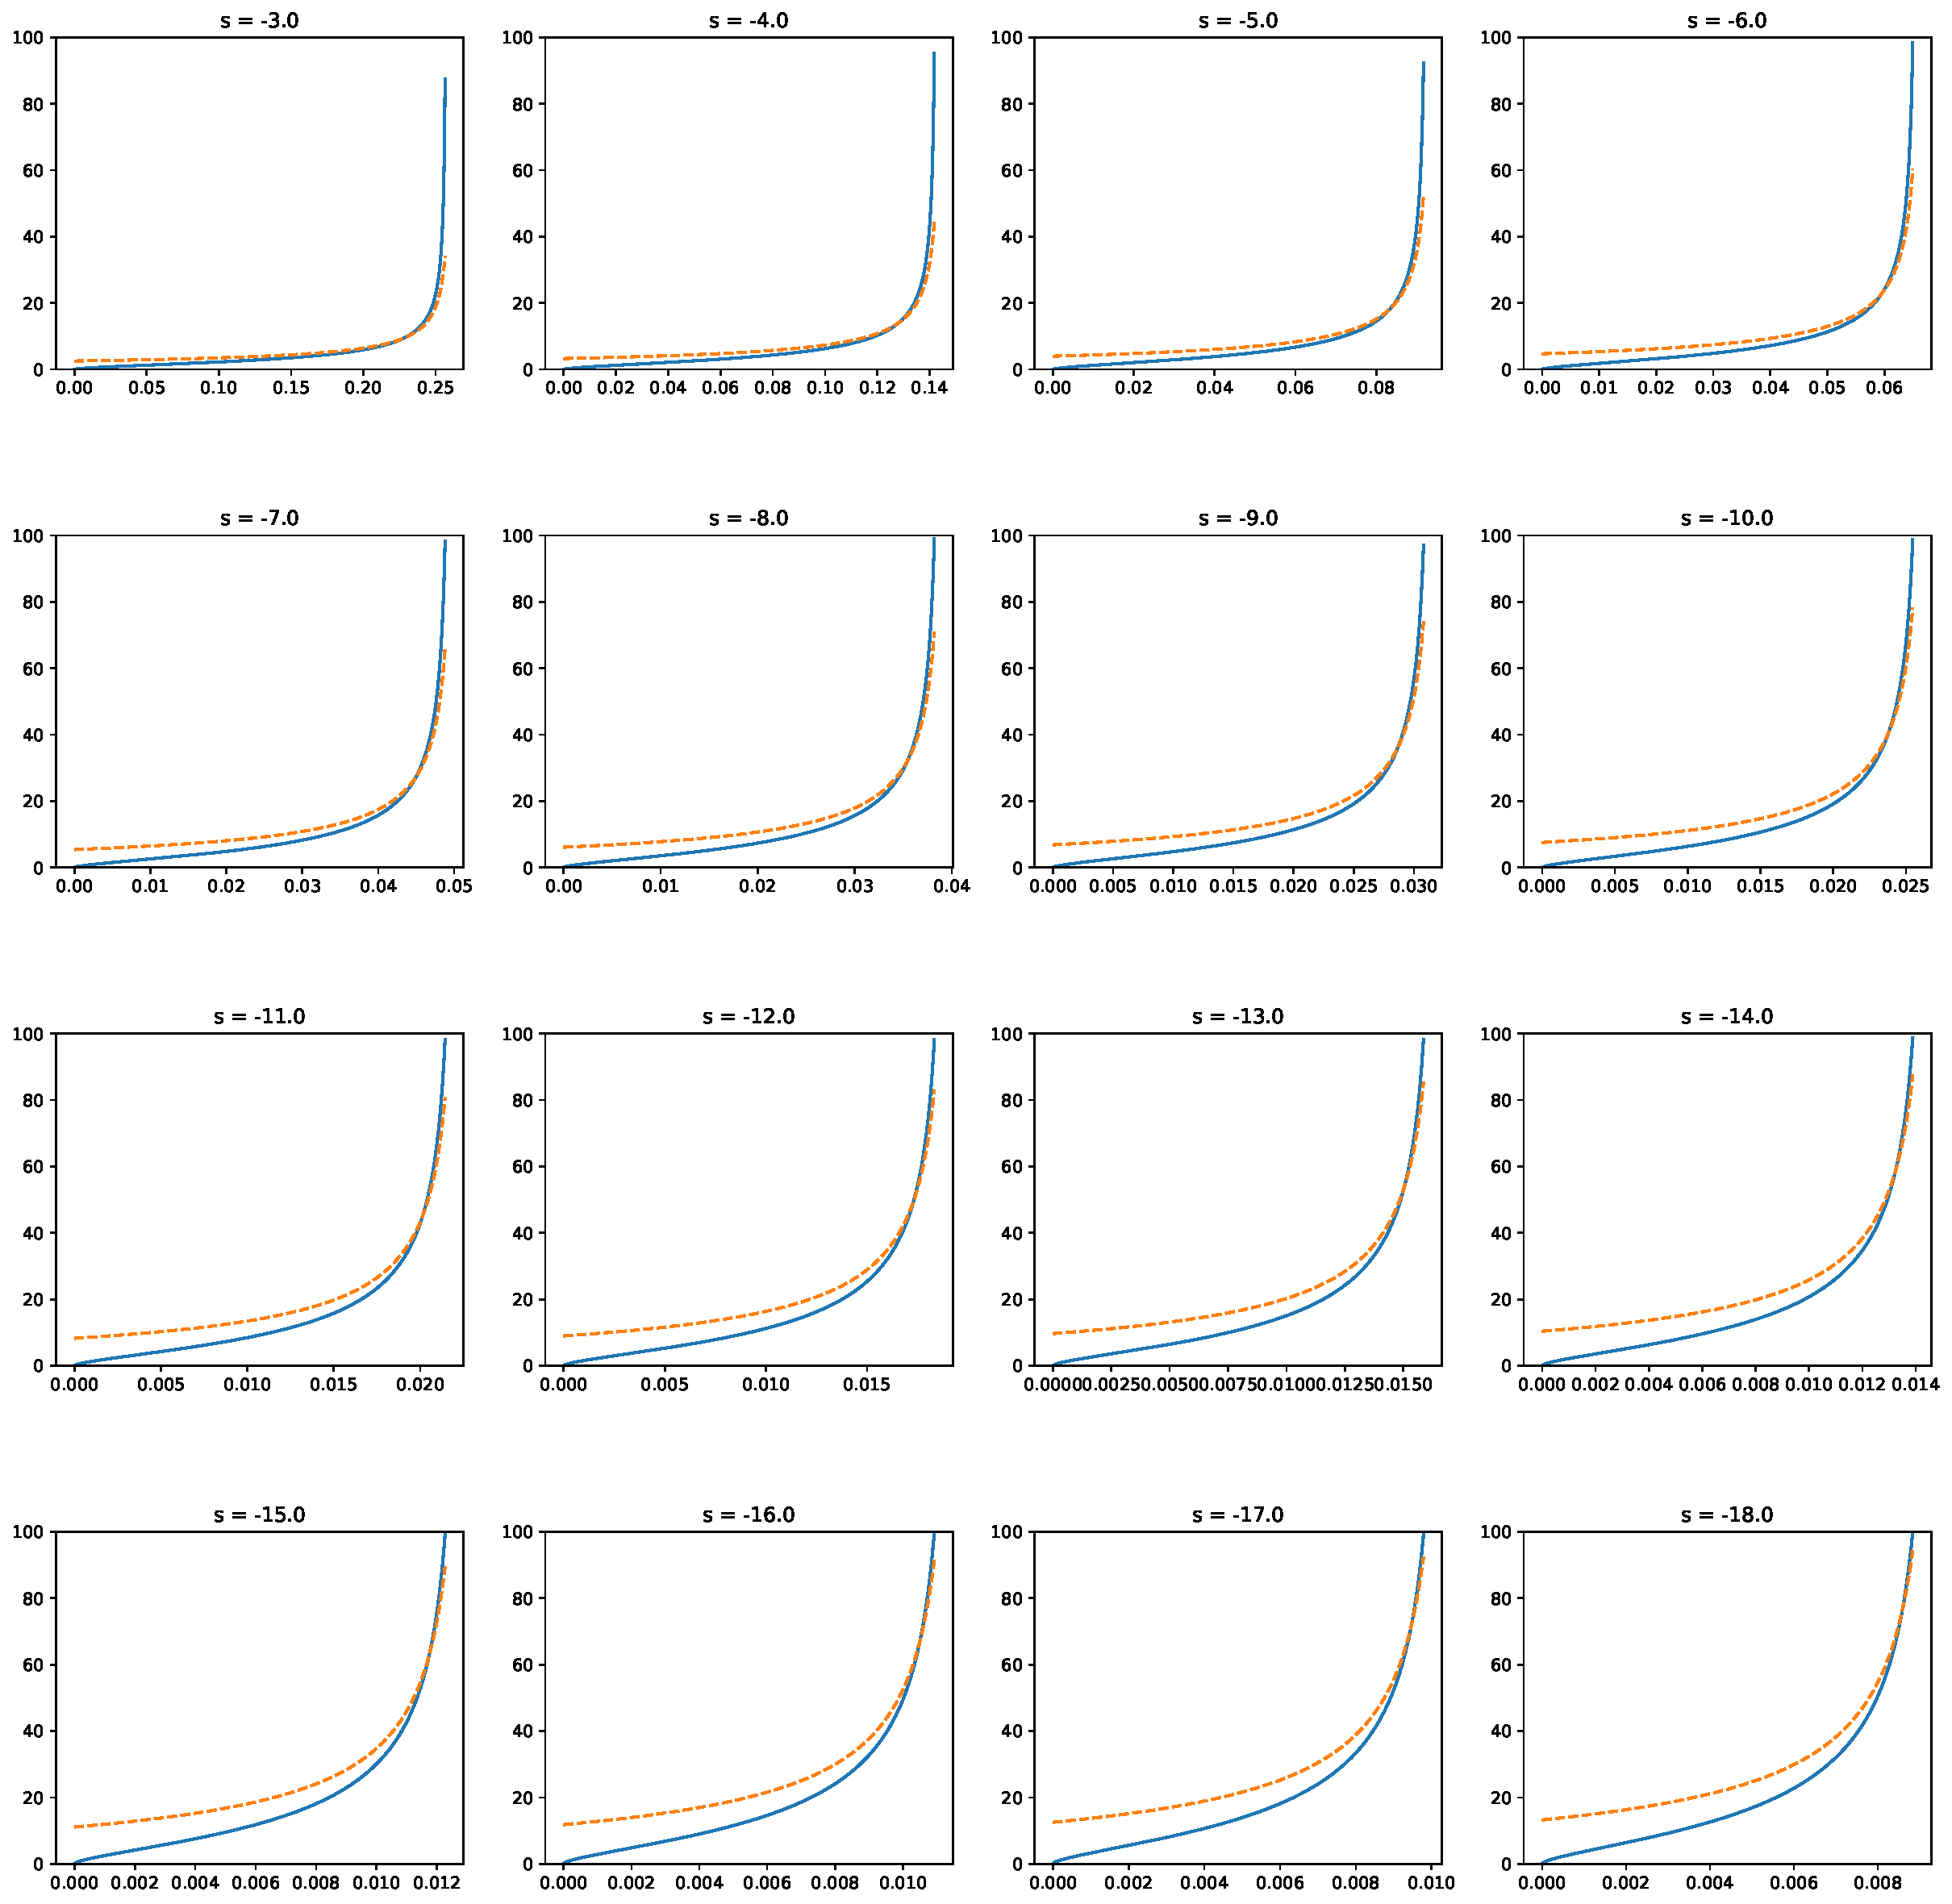
\includegraphics[width=\textwidth]{figures/FractionalRiccatiApproximationNegativeCorrelation.pdf}
    \caption{Solution of the fractional Riccati equation (blue) and approximation (orange) for model parameters $\alpha=0.6$, $\lambda=2$, $\rho = -0.8$, $\xi = 1$.}
    \label{fig:FractionalRiccatiApproximationNegativeCorrelation}
\end{figure}

Figure \ref{fig:FractionalRiccatiApproximationNegativeCorrelation} demostrates solution of the fractional Riccati equation and approximation from previous section with negative correlation. For this choice of parameters explosion times are known explicitly from \cite{GGP18} for $s \leq 2.5$. Since the correlation is negative, spot and variance balance each other out and hence spot is more likely to go to zero rather than explode. Hence the explosive moments are negative.

\begin{figure}[H]
    \centering
    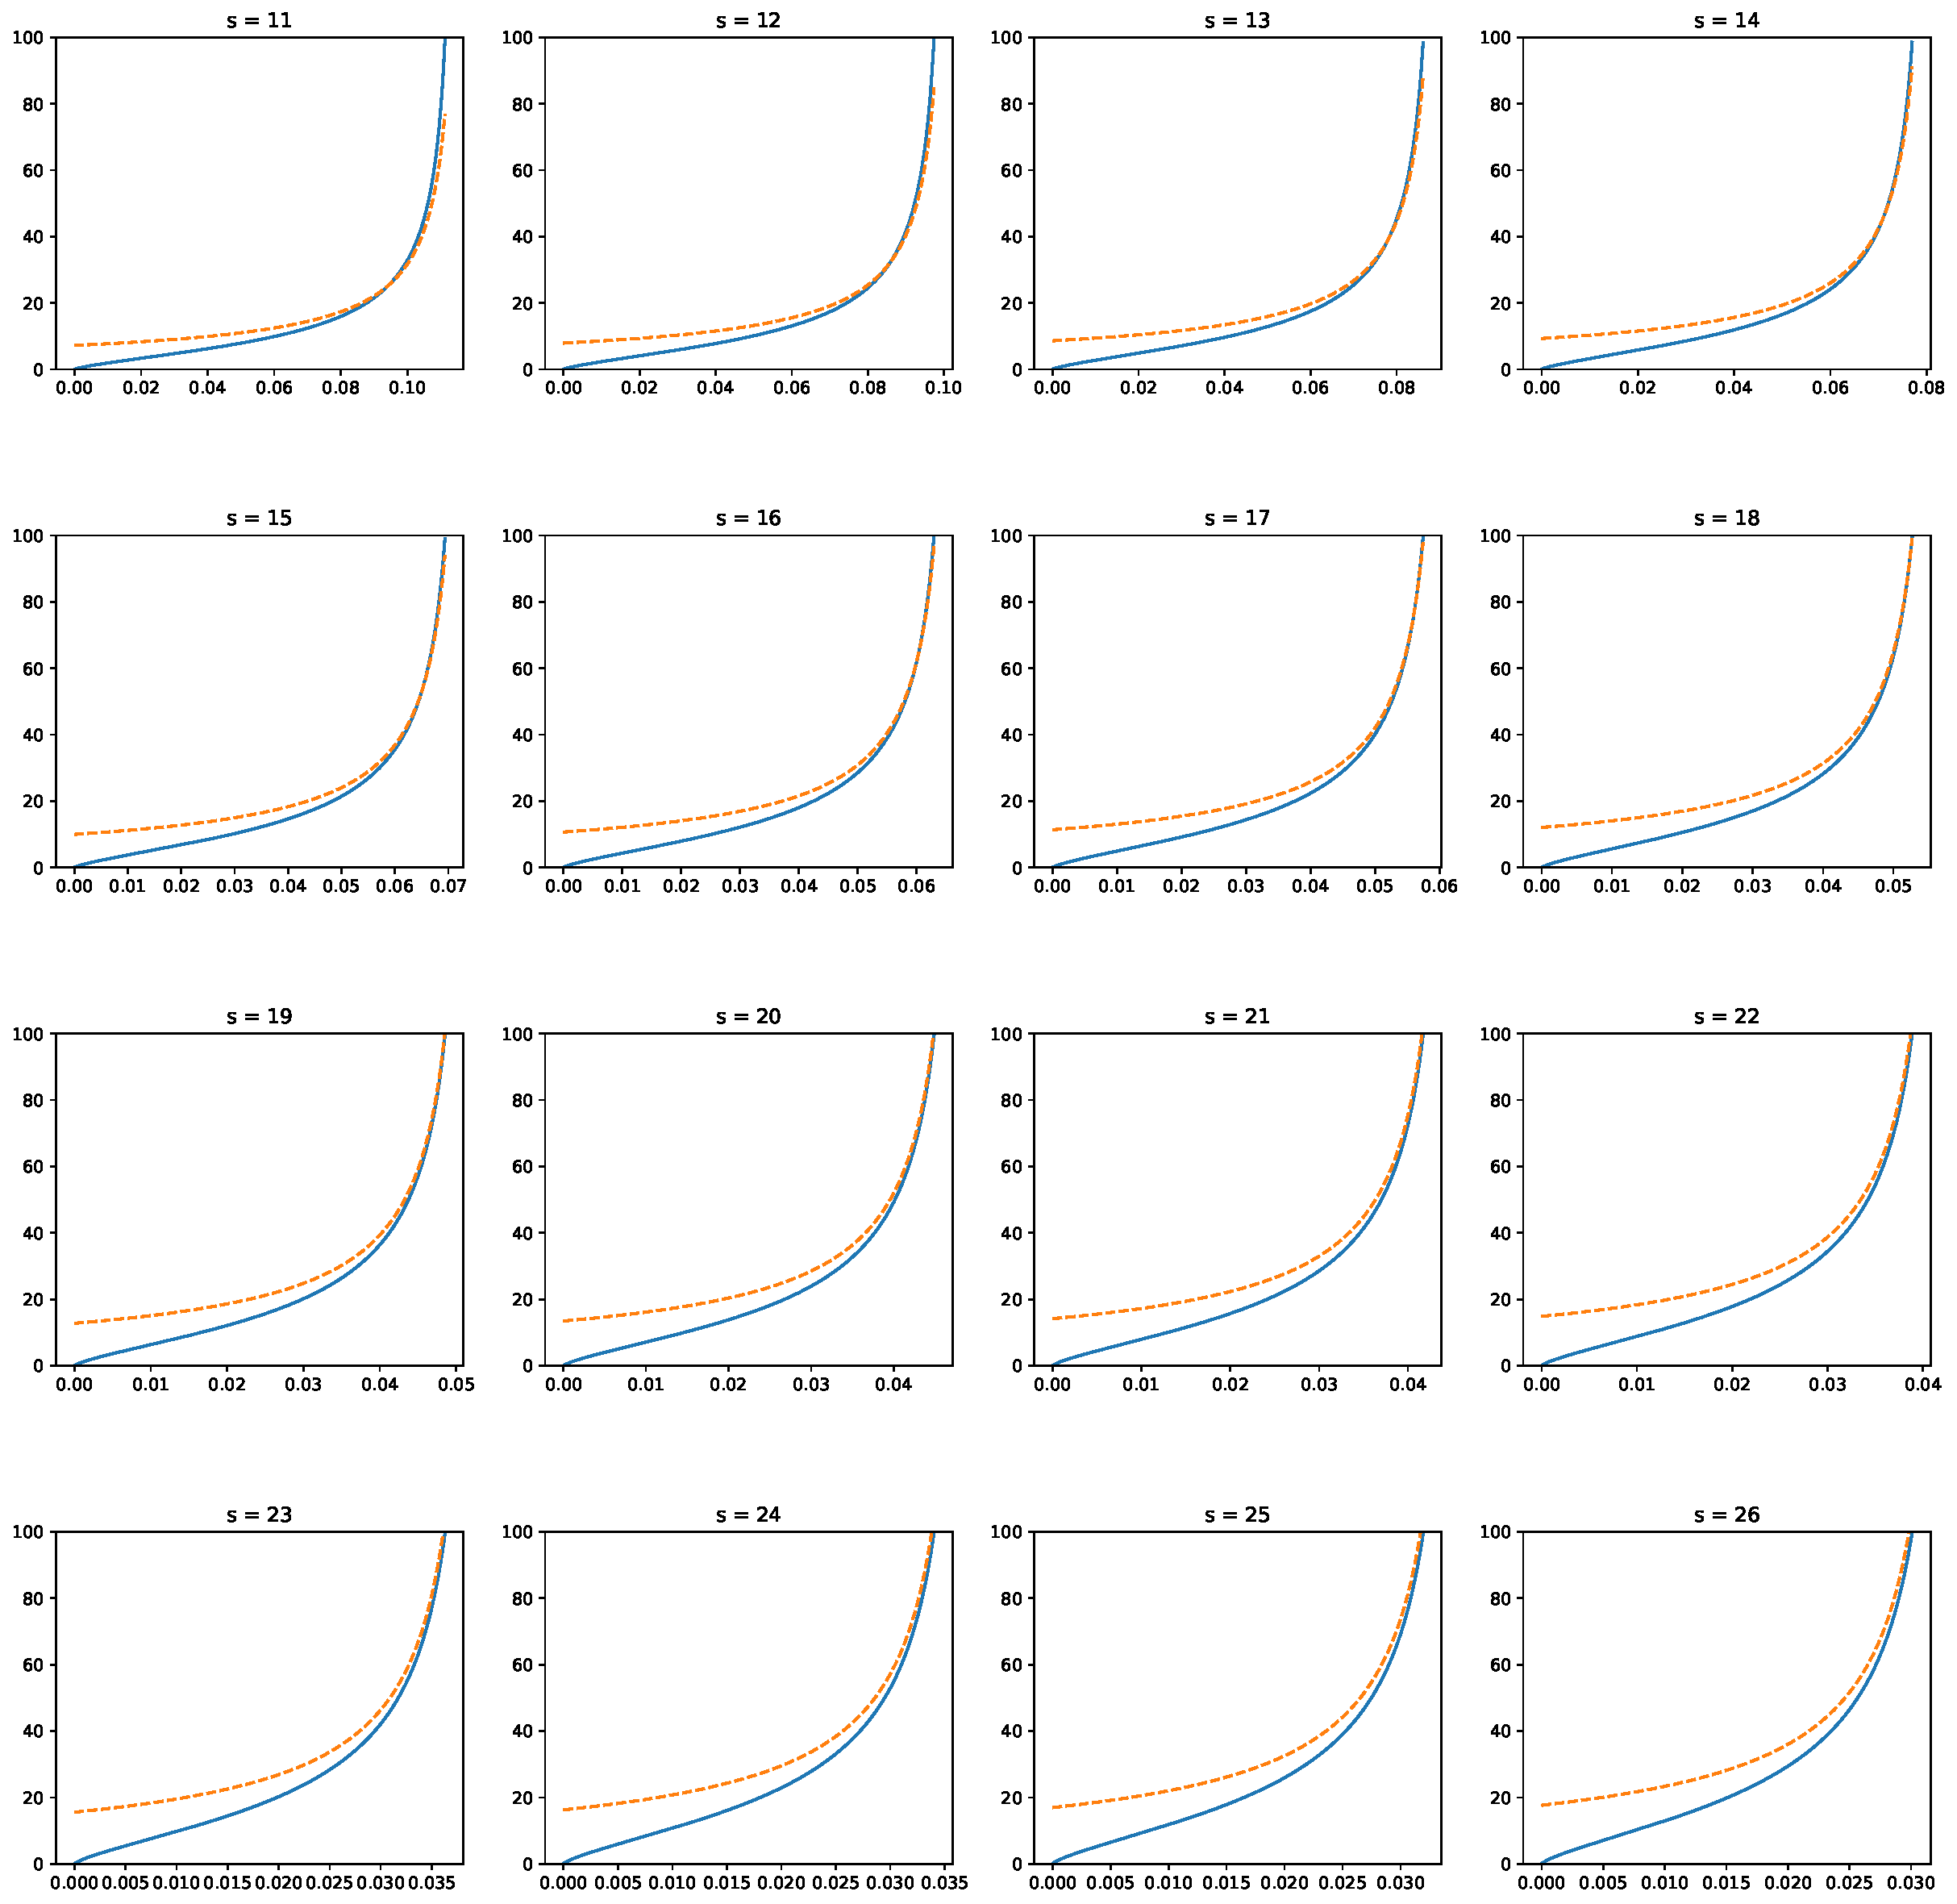
\includegraphics[width=\textwidth]{figures/FractionalRiccatiApproximationPositiveCorrelation.pdf}
    \caption{Solution of the fractional Riccati equation (blue) and approximation (orange) for model parameters $\alpha=0.75$, $\lambda=1$, $\rho = 0.1$, $\xi = 1$.}
    \label{fig:FractionalRiccatiApproximationPositiveCorrelation}
\end{figure}

Figure \ref{fig:FractionalRiccatiApproximationPositiveCorrelation} demostrates solution of the fractional Riccati equation and approximation from previous section with positive correlation. For this choice of parameters explosion times are known explicitly from \cite{GGP18} for $s \geq 10$. Since the correlation is positive, spot and variance reinforce each other and hence spot is more likely to explode rather than go to zero. Hence the explosive moments are positive.

We see that in both cases asymptotic behavior of the numerical solution coincides with the approximation from the previous section.

\section{Expansion of the Rough Heston log-mgf}

\subsection{Expansion of the log-mgf near blow-up}

Recalling the definition \eqref{mellin w} of $w(\eta)$ we obtain expansion of the solution of the original equation near blow-up $t \uparrow T^*$

\begin{equation}\label{psiexpansion}
\begin{aligned}
\psi(s, t) &= \frac{\Gamma(2\alpha)}{\frac 12 \xi^2 \Gamma(\alpha)} \left(T^*-t\right) ^{-\alpha} + \frac{\Gamma'(\alpha)}{\Gamma(\alpha)^2} \left(\frac{\rho\xi s - \lambda}{\frac{\Gamma(\alpha)}{\Gamma(2\alpha)} - \xi^2} \right) + O((T^* - t)^{\alpha})\\[10pt]
&= \Theta_0 (T^*-t)^{-\alpha} + \Theta_1 + O((T^*-t)^\alpha)
\end{aligned}
\end{equation}

Turning back to the formula \eqref{logmgf}, we want to consider asymptotics of $I^1\psi$ and $I^{1-\alpha}\psi$. We note that

\begin{equation}\label{i1expansion}
\begin{aligned}
I^1\psi(s,t) &= \int _0 ^t \psi(s, \tau) d\tau\\[10pt]
&= \int _0^t\left[\psi(s,\tau) - \Theta_0 (T^*-\tau)^{-\alpha} + \Theta_0(T^*-\tau)^{-\alpha}\right] d\tau\\[10pt]
&= \int _0^{T^*} \left[\psi(s,\tau)  - \Theta_0(T^*-\tau)^{-\alpha}\right] d\tau + \Theta_0 T^{*}^{(1-\alpha)} \\
&\qquad + \Theta_0 (T^*-t)^{1-\alpha} + O(T^*-t)\\[10pt]
&=: A+K +O(T^*-t)
\end{aligned}
\end{equation}

where the have the constant term, term of the order $1-\alpha$ and the rest. In particular, no contribution to the explosion of the log-mgf from this part.

On the other hand, we have

\begin{equation} \label{i1alphaexpansion}
\begin{aligned}
I^{1-\alpha}\psi(s,\tau) &= \frac{1}{\Gamma(1-\alpha)} \int _0 ^t (t-\tau)^{-\alpha} \psi(s, \tau) d\tau\\[10pt]
&= \frac{1}{\Gamma(1-\alpha)} \int _0^t(t-\tau)^{-\alpha}\left[\psi(s,\tau) - \Theta_0 (T^*-\tau)^{-\alpha} \right] d\tau\\
&\qquad + \frac{1}{\Gamma(1-\alpha)} \int _0^t(t-\tau)^{-\alpha}\left[\Theta_0(T^*-\tau)^{-\alpha}\right] d\tau\\[10pt]
&= \frac{1}{\Gamma(1-\alpha)} \int _0^{T^*}(t-\tau)^{-\alpha}\left[\psi(s,\tau) - \Theta_0(T^*-\tau)^{-\alpha} \right] d\tau\\
&\qquad + \frac{1}{\Gamma(1-\alpha)} \int _0^t(t-\tau)^{-\alpha}\left[\Theta_0(T^*-\tau)^{-\alpha}\right] d\tau + O(T^*-t)\\[10pt]
&=:B+L + O(T^*-t)
\end{aligned}
\end{equation}

The term $B$ will again make a contribution of the constant order and higher, whereas the term $L$ is explosive.

We can expand around $T^*$

$$
(t-\tau)^{-\alpha} = \sum_{k=0}^\infty \frac{(-1)^{k+1}}{k!}\left\{\frac{\alpha \cdot (\alpha + 1) \cdots (\alpha+k-1)}{(T^*-\tau)^{\alpha+k}} \right\} (T^*-t)^k
$$

and termwise integration yields

$$
\begin{aligned}
&\int_0^t (t-\tau)^{-\alpha}(T^*-\tau)^{-\alpha} d\tau\\[5pt] &\qquad=(T^*-t)^{1-2\alpha}\sum_{k=0}^\infty \frac{(-1)^{k}}{k!}\left\{\frac{\alpha \cdot (\alpha + 1) \cdots (\alpha+k-1)}{2\alpha+k-1} \right\}
+ \frac{(T^*)^{1-2\alpha}}{1-2\alpha} + O(T^*-t)\\[5pt]
&\qquad=(T^*-t)^{1-2\alpha}\sum_{k=0}^\infty \frac{(-1)^{k}}{B(\alpha, k)}\left\{\frac{1}{2\alpha+k-1} \right\} + \frac{(T^*)^{1-2\alpha}}{1-2\alpha} + O(T^*-t).
\end{aligned}
$$

The series in the above expansion is convergent for $\alpha \in (\frac 12, 1)$ and can be expressed in terms of the incomplete beta function

$$
\sum_{k=0}^{\infty} \frac{(-1)^{k}}{2 \alpha+k-1}\left\{\frac{\alpha \cdot(\alpha+1) \cdots(\alpha+k-1)}{k !}\right\}=-(-1)^{-2\alpha} \beta_{-1}(2 \alpha-1,1-\alpha)
$$

Hence we obtain

$$
\begin{aligned}
L &= \frac{\Theta_0}{\Gamma(1-\alpha)} \left[
-(-1)^{-2\alpha} \beta_{-1}(2 \alpha-1,1-\alpha)\right] (T^*-t)^{1-2\alpha}\\[10pt]
&\qquad+\frac{\Theta_0}{\Gamma(1-\alpha)} \left[
\frac{(T^*)^{1-2\alpha}}{1-2\alpha}\right] + O(T^*-t)
\end{aligned}
$$

which gives us the term of order $1-2\alpha < 0$, the constant term and the rest.

Plugging the expansions \eqref{i1expansion} and \eqref{i1alphaexpansion} into the definition \eqref{logmgf} of the Heston log-mgf we obtain

\begin{equation}\label{logmgfexpansion}
\begin{aligned}
m(s, t) &= \Lambda_0 (T^*-t)^{1-2\alpha}
+ \Lambda_1 + \Lambda_2 (T^*-t)^{1-\alpha} + O(T^*-t)
\end{aligned}
\end{equation}

for the constants

\iffalse
$$
\begin{aligned}
\Lambda_0 &= \frac{v_0 \Gamma(2\alpha)}{\frac 12 \xi ^2 \Gamma(1-\alpha)\Gamma(\alpha)} \left[
-(-1)^{-2\alpha} \beta_{-1}(2 \alpha-1,1-\alpha)\right]\\[10pt]
\Lambda_1 &= \frac{v_0\Gamma(2\alpha)}{\frac 12 \xi ^2 \Gamma(1-\alpha)\Gamma(\alpha)} \left[
\frac{(T^*)^{1-2\alpha}}{1-2\alpha}\right]+ \bar v \lambda\frac{\Gamma(2\alpha)}{\frac 12 \xi ^2 \Gamma(\alpha) } T^{*}^{(1-\alpha)}\\
&\qquad + \bar v \lambda \int _0^{T^*} \left[\psi(u,s)  - \frac{\Gamma(2\alpha)}{\frac 12 \xi ^2 \Gamma(\alpha) }(T^*-s)^{-\alpha}\right] ds \\
&\qquad +  \frac{v_0}{\Gamma(1-\alpha)} \int _0^{T^*}(t-s)^{-\alpha}\left[\psi(u,s) - \frac{\Gamma(2\alpha)}{\frac 12 \xi ^2 \Gamma(\alpha) }(T^*-s)^{-\alpha} \right] ds\\[10pt]
\Lambda_2 &= \frac{\bar v \lambda \Gamma(2\alpha)}{\frac 12 \xi ^2 \Gamma(\alpha) }
\end{aligned}
$$
\fi

$$
\begin{aligned}
\Lambda_0 &= \frac{v_0 \Theta_0}{\Gamma(1-\alpha)} \left[
-(-1)^{-2\alpha} \beta_{-1}(2 \alpha-1,1-\alpha)\right]\\[10pt]
\Lambda_1 &= \frac{v_0\Theta_0}{\Gamma(1-\alpha)} \left[
\frac{(T^*)^{1-2\alpha}}{1-2\alpha}\right]+ \bar v \lambda\Theta_0 T^{*}^{(1-\alpha)}\\
&\qquad + \bar v \lambda \int _0^{T^*} \left[\psi(s,\tau)  - \Theta_0(T^*-\tau)^{-\alpha}\right] d\tau \\
&\qquad +  \frac{v_0}{\Gamma(1-\alpha)} \int _0^{T^*}(t-\tau)^{-\alpha}\left[\psi(s,\tau) - \Theta_0(T^*-\tau)^{-\alpha} \right] d\tau \\[10pt]
\Lambda_2 &= \bar v \lambda \Theta_0.
\end{aligned}
$$

Observe that $\Lambda_1$ is indeed integrable since we removed singularity of the log-mgf from the integrands.

\subsection{Expansion around the critical moment}

Until now, we kept the moment $s$ and critical time $T^*$ fixed.

We now define the function $T^*(s)$ to be the moment explosion time

$$
T^{*}(s):=\sup \left\{t \geq 0: \mathbb{E}\left[e^{s X_{t}}\right]<\infty\right\}.
$$

Let's assume that $T^*$ is twice continuously differentiable, and denote by $\sigma := -T^*(s_+)'$ and $\kappa := T^*(s_+)''$ the first and second derivatives of the critical moment, respectively. We can then write

$$
\begin{aligned}
(T^*-t)^{1-2\alpha} &= \left[\sigma (s_+ -s) + \frac \kappa 2 (s_+ - s)^2 + O(s_+-s)^3 \right]^{1-2\alpha}\\[5pt]
&=\sigma^{1-2\alpha}(s_+-s)^{1-2\alpha} + \frac{\kappa(1-2\alpha)}{2\sigma^{-2\alpha}} (s_+-s)^{2-2\alpha} + O(s_+-s)^{3-2\alpha}\\[20pt]
(T^*-t)^{1-\alpha}&=\left[\sigma (s_+ -s) + \frac \kappa 2 (s_+ - s)^2 + O(s_+-s)^3 \right]^{1-\alpha}\\[5pt]
&=\sigma^{1-\alpha}(s_+-s)^{1-\alpha}+\frac{\kappa(1-\alpha)}{2\sigma^{-\alpha}}(s_+-s)^{2-\alpha} + O(s_+-s)^{3-\alpha}
\end{aligned}
$$

We can now express the expansion in terms of the critical moment $s_+$

\begin{equation}\label{logmgfcriticalexpansion}
\begin{aligned}
m(s,t)&=\Lambda_0 \sigma^{1-2\alpha}(s_+-s)^{1-2\alpha} + \Lambda_1 + \Lambda_2\sigma^{1-\alpha}(s_+-s)^{1-\alpha} \\[5pt]
&\qquad+ \Lambda_0 \frac{\kappa (1-2\alpha)}{2\sigma^{-2\alpha}}(s_+-s)^{2-2\alpha} + O(s_+-s).
\end{aligned}
\end{equation}

\section{Expansion of the Rough Heston density}

Basically we want to justify the step

$$
\int_{\hat s-i\infty}^{\hat s + i\infty} e^{-ks} M(s,T)ds \sim \int_{\hat s -ih(k)}^{\hat s + ih(k)} e^{-ks} M(s,T)ds
$$

for $h(k)$ small as $k\rightarrow \infty$, which would mean that in complete analogy to the Heston case, the main contribution to the integral comes from the part where the mgf features exponential explosion.

\begin{remark}
In the Mellin domain, we denote the variable $u$ instead of $s$ and work with $u_* = s_+ +1$.
\end{remark}

\subsection{Approximate saddlepoint}

\begin{proposition}
Approximate saddle point is given by

\begin{equation} \label{approximatesaddlepoint}
u_* - \hat u \sim \beta k ^{-\frac{1}{2\alpha}}
\end{equation}

with $\beta = \left(\Lambda_0(2\alpha -1) \sigma ^ {1-2\alpha}\right)^{\frac{1}{2\alpha}}$

\end{proposition}

\begin{proof}

Remember the saddle point equation $\frac{\partial}{\partial u}m(\hat u - 1, T) = k$. Using \eqref{logmgfcriticalexpansion}, we obtain

$$
\begin{aligned}
m(u - 1,t)&\sim \Lambda_0 (\sigma(u_*-u))^{1-2\alpha}\\
\frac{\partial}{\partial u} m(u-1,t) &\sim - \Lambda_0 (1-2\alpha) \sigma^{1-2\alpha} (u_*-u)^{-2\alpha}\\
u_*-\hat u &\sim \beta k ^{-\frac{1}{2\alpha}}
\end{aligned}
$$

\end{proof}

\subsection{Local expansion around the saddle point}

Previously we obtained expansion of the log-mgf around the critical moment. Using the asymptotic \eqref{approximatesaddlepoint} of the approximate saddle point, we now want to obtain expansion of the log-mgf around the approximate saddle point $\hat u$ in terms of the asymptotic parameter $k\rightarrow \infty$.

Consider $u = \hat u + iy$ and $|y|<k^{-\gamma}$ for $\frac{\alpha+1}{3\alpha}< \gamma < \frac{3}{4\alpha} $. Then $u_*-u=\beta k^{-\frac{1}{2\alpha}}$ and we can write

$$
\begin{array}{ll}
(u_*-u)^{1-2\alpha} &= \beta^{1-2\alpha}k^{1-\frac{1}{2\alpha}} + iy\beta^{-2\alpha}(2\alpha-1)k - \beta^{-1-2\alpha}y^2 k^{1+\frac{1}{2\alpha}} + O(k^{1+\frac 1\alpha -3\gamma})\\[5pt]
(u_*-u)^{1-\alpha} &= \beta^{1-\alpha}k^{\frac 12-\frac{1}{2\alpha}} + iy\beta^{-\alpha}(2\alpha-1)k^{\frac 12} - \beta^{-1-\alpha}y^2 k^{\frac 12+\frac{1}{2\alpha}} + O(k^{\frac 12+\frac 1\alpha-3\gamma})\\[5pt]
(u_*-u)^{2-2\alpha} &= \beta^{2-2\alpha}k^{1-\frac{1}{\alpha}} + iy\beta^{1-2\alpha}(2\alpha-1)k^{1-\frac{1}{2\alpha}} - \beta^{-2\alpha}y^2k + O(k^{1+\frac {1}{2\alpha}-3\gamma})
\end{array}
$$

By our choice of $\gamma$, the asymptotic terms are $o(1)$. Moreover, by our choice of $y$, all contributions from $(u_*-u)^{2-2\alpha}$ and $(u_*-u)^{1-\alpha}$ are $O(L^{1+\frac 1\alpha -3\gamma})$ (and in particular $o(1)$). Hence we obtain the expansion around the saddle point

\begin{equation}\label{logmgfexpansionaroundthesaddlepoint}
\begin{aligned}
m(\hat u - 1 + iy,t)&=\Lambda_0\sigma^{1-2\alpha}\beta^{1-2\alpha}k^{1-\frac{1}{2\alpha}} + iyk - \Lambda_0 \sigma ^{1-2\alpha} \beta^{-1-2\alpha} y^2 k^{1 + \frac{1}{2\alpha}} \\
&\qquad+ \Lambda_1 + O(k^{1+\frac 1\alpha -3\gamma})\\[10pt]
&=\frac{\beta}{2\alpha - 1} k ^ {1-\frac{1}{2\alpha}} + iyk - \frac{\beta^{-1}}{2\alpha - 1} k ^{1+\frac{1}{2\alpha}} y^2 + \Lambda_1+ O(k^{1+\frac 1\alpha -3\gamma})
\end{aligned}
\end{equation}

\subsection{Saddle point approximation of the density}

We first want to show that the tails are exponentially small and hence can be neglected.

\begin{proposition}\label{tailasymptotic}

Rough Heston mgf satisfies

$$
\left|e^{\bar{v} \lambda I^{1} \psi(u, t)+v_{0} I^{1-\alpha} \psi(u, t)}\right|=O\left(e^{-C \Im(u)}\right).
$$

where the constant $C$ depends on $t$ and $v_0$.

\end{proposition}

\begin{proof}

We proceed along the lines of the proof of Lemma 18 in \cite{FGGS10}.

We write $\psi = f + ig$ and investigate the real part $f$ for the absolute value above since

$$
\left|e^{v_{0} \psi(u, T)}\right|=e^{v_{0} f(u, T)}.
$$

We write $u=x+iy$ and $\gamma = -(\rho \xi u - \lambda)$. The real and imaginary part satisfy the equations

$$
\[\arraycolsep=20pt
\begin{array}{ll} D^\alpha f =\frac{1}{2}\left(x^{2}-y^{2}-x\right)+\frac{\xi^{2}}{2}\left(f^{2}-g^{2}\right)-\gamma f & f(u, 0)=0 \\[10pt] D^\alpha g =\frac{1}{2}(2 \xi y-y)+\xi^{2} f g-\gamma g & g(u, 0)=0 \end{array}
\]
$$

Further we see

$$
\begin{aligned} D^\alpha f & \leq \frac{1}{2}\left(x^{2}-y^{2}-x\right)+\frac{\xi^{2}}{2} f^{2}-\gamma f \\ & \leq-\frac{1}{3} y^{2}+\frac{\xi^{2}}{2} f^{2}-\gamma f =: V(y,f). \end{aligned} 
$$

From the proof of Lemma 18 in \cite{FGGS10} we have

$$
V(y, F) \leq \dot{F}
$$

for the function $F(y,t):=-yC(t)$ with

$$
C(t)=\left\{\begin{array}{ll}{\theta \gamma^{-1}\left(1-e^{-\gamma t}\right)} & {\text { if } \gamma>0} \\ {\theta t} & {\text { if } \gamma=0}\end{array}\right.
$$

for $\theta>0$ such that $-\frac{1}{3}+\frac{\xi^{2}}{2} T^{2} \theta^{2}=-\frac{1}{4}$ and $y$ large enough.

Define $h(t) := f(s,t) - D^{1-\alpha} F(s,t)$. Assume $\exists b > 0:h(b)>0$. Then $\exists c\in(0,b) : h(c)=0$ and  $\forall x \in (c,b]$ we have $h(x)>0$. Since the function $V$ is locally Lipschitz, we obtain

$$
\begin{aligned}
D^\alpha h(x) & \leq V(s, f(s,x)) - V(s, F(s,x))\\[5pt]
&\leq L|f(s,x)-F(s,x)|\\[5pt]
&=Lh(x).
\end{aligned}
$$

Finally, with Gronwall lemma we get

$$
h(b)\leq \frac{L}{\Gamma(\alpha)}\int _c^b(x-s)^{\alpha-1}h(s)ds\qquad \Rightarrow \qquad h(b) \leq 0.
$$

which is a contradiction. Therefore we can write

$$
f(s, t)\leq D^{1-\alpha} F(y,t)
$$

Fractional differentiation of the power series of $C(t)$ yields

$$
D^{1-\alpha}F(y, t) = -y\left(\frac \theta \gamma\right) \frac{1}{t^{1-\alpha}} E_{1,\alpha}(-\gamma t)=:-C \Im(u) k(t)
$$

for $\varphi(t):=\frac{1}{t^{1-\alpha}} E_{1,\alpha}(-\gamma t)$. Once we ensure that $I^{1-\alpha}\varphi$ and $I^1\varphi$ are integrable for fixed $y$, the constant can be fixed and we are done.

\end{proof}

We first consider estimate of the tails $\Im (u) > B$ for fixed $B>0$, and then establish the asymptotic for $\Im (u) > k^{-\gamma}$.

\begin{proposition}

Let $B>0$. Then

$$
\left|\int_{\hat{u}+i B}^{\hat{u}+i \infty} e^{-ku+\bar{v} \lambda I^{1} \psi(u-1, t)+v_{0} I^{1-\alpha} \psi(u-1, t)} d u\right|=O\left(\exp \left(-ku_* +\beta k^{1 -\frac{1}{2\alpha}}\right)\right)
$$

\end{proposition}

\begin{proof}
For $\tilde B \gg B$ large enough, the asymptotic for the portion of the integral from $\tilde B$ to $\infty$ follows from the expansion \eqref{logmgfexpansionaroundthesaddlepoint} and the previous proposition.

For the portion between $B$ and $\tilde B$ the asymptotic follows again from the expansion \eqref{logmgfexpansionaroundthesaddlepoint} and the fact that we integrate away from zero, hence the Gaussian integral in the resulting expansion will converge to 1.
\end{proof}

We now establish the tail estimate for $k^{-\gamma}$.

\begin{proposition}\label{tailestimate}

The tail can be estimated by

$$
\left|\int_{\hat u +i k^{-\gamma}} ^{\hat u + i \infty} \exp(-ku + m(u-1,t))du\right|=\exp\left(-ku_* + \frac{2\alpha\beta}{2\alpha-1} k^{1-\frac{1}{2\alpha}}+  \alpha\beta^{-1}k^{1+\frac{1}{2\alpha} -2\gamma} + O(k^{1+\frac{3}{2\alpha} - 4\gamma}) \right)
$$

\end{proposition}

\begin{proof}

From the expansion \eqref{logmgfcriticalexpansion} around critical moment we know that

$$
m(u-1,t) &= \frac{\beta^{2\alpha}}{2\alpha-1}(u_*-u)^{1-2\alpha} + O(1)
$$

Hence in the vicinity of $u_+$ inside the analyticity strip, i.e. $\exists B>0: \Im(u)<B, u_*-B<\Re(u)$ we can estimate

$$
|M(u-1,t)|&\leq C\exp\left(\frac{\beta^{2\alpha}}{2\alpha-1}(u_*-u)^{1-2\alpha}\right).
$$

for some constant $C>0$. Passing to the integral we obtain

$$
\begin{aligned}
&\left|\int_{\hat u +i k^{-\gamma}} ^{\hat u + i B} \exp(-ku + m(u-1,t))du\right|\\
&\qquad \leq C\exp(-ku_* + \beta k^{1-\frac{1}{2\alpha}}) \int _{k^{-\gamma}} ^ B \exp\left( \Re \left\{ \frac{\beta ^ {2\alpha}}{2\alpha - 1} (u_*-(\hat u + iy)) ^{1-2\alpha} \right\}\right)dy\\
&\qquad \leq C\exp\left(-ku_* + \beta k^{1-\frac{1}{2\alpha}}+ \Re \left\{ \frac{\beta ^ {2\alpha}}{2\alpha - 1} (u_*-(\hat u + i k^{-\gamma})) ^{1-2\alpha} \right\} \right)\\
&\qquad = C\exp\left(-ku_* + \beta k^{1-\frac{1}{2\alpha}}+ \frac{\beta}{2\alpha-1}k^{1-\frac{1}{2\alpha}} - \alpha\beta^{-1}k^{1+\frac{1}{2\alpha} -2\gamma} + O(k^{1+\frac{3}{2\alpha} - 4\gamma}) \right)\\
&\qquad = C\exp\left(-ku_* + \frac{2\alpha\beta}{2\alpha-1} k^{1-\frac{1}{2\alpha}}-  \alpha\beta^{-1}k^{1+\frac{1}{2\alpha} -2\gamma} + O(k^{1+\frac{3}{2\alpha} - 4\gamma}) \right)
\end{aligned}
$$

where we used H{\"o}lder inequality in the second inequality and the expansion

$$
\begin{aligned}
\frac{\beta^{2\alpha}}{2\alpha-1}\Re\left\{(u_*-(\hat u + ik^{-\gamma}))^{1-\alpha}\right\} = \frac{\beta}{2\alpha-1}k^{1-\frac{1}{2\alpha}} - \alpha \beta^{-1}k^{1+\frac{1}{2\alpha}-2\gamma} + O(k^{1+\frac{3}{2\alpha}-4\gamma})
\end{aligned}
$$

right after that.

Since $B>0$, it follows from Proposition \ref{tailasymptotic} that portion of the integral $\int_{\hat u +i B} ^{\hat u + i \infty} \exp(-ku + m(u-1,t))du$ is asymptotically smaller than $\int_{\hat u +i k^{-\gamma}} ^{\hat u + i B} \exp(-ku + m(u-1,t))du$.

\end{proof}

We are now ready to deal with the expansion of the Rough Heston density.

\begin{proposition}

Asymptotics of the Rough Heston density is given by

$$
\frac{\exp\left(\Lambda_1\right)}{2\pi} \sqrt {\pi\beta(2\alpha-1)} \exp\left(-k u_* +  \frac{2\beta}{2\alpha - 1}k^{1-\frac{1}{2\alpha}}\right) k^{-\frac 12 -\frac{1}{4\alpha}} \left(1+O(k^{1-\frac 54 \alpha + \varepsilon})\right)
$$

for any $\varepsilon > 0$.

\end{proposition}

\begin{proof}

We start by shifting the contour to the approximate saddle point $\hat u$ in order to proceed with Laplace method for contour integrals. We obtain the density as inverse Mellin transform

$$
\begin{aligned}
D_t(k) &= \frac{1}{2\pi i} \int_{\hat u -i\infty}^{\hat u + i\infty} e^{-ku+\bar{v} \lambda I^{1} \psi(u-1, t)+v_{0} I^{1-\alpha} \psi(u-1, t)}du \\[10pt]
&=\frac{e^{-k\hat u}}{2\pi } \int_{-\infty}^{ + \infty} e^{-iyk+m(\hat u + iy - 1, t)}du\\[10pt]
&=\frac{e^{-k\hat u}}{2\pi } \int_{-k^{-\gamma}}^{ k^{-\gamma}} e^{-iyk+m(\hat u + iy - 1, t)}du + \text{tails}\\[10pt]
&=:I+J
\end{aligned}
$$

Note that $k\hat u = k u_* + \beta k ^{1-\frac{1}{2\alpha}}$. Hence the first part can be calculated explicitly from the expansion \eqref{logmgfexpansionaroundthesaddlepoint}

$$
\begin{aligned}
I &= \frac{e^{-k\hat u}}{2\pi} \int_{-k^\gamma}^{ k^\gamma} e^{-iyk+m(\hat u + iy - 1, t)}du\\
&=\frac{e^{-k u_*}}{2\pi}\exp\left(\Lambda_1 + \frac{2\beta}{2\alpha - 1}k^{1-\frac{1}{2\alpha}}\right)\left\{\int _{-k^\gamma} ^{k^\gamma} \exp\left(-\frac{\beta^{-1}}{2\alpha-1} k ^{1+\frac{1}{2\alpha}} y^2\right) dy\right\} \left(1+O(k^{1+\frac 1\alpha -3\gamma})\right)\\[5pt]
&=\frac{e^{-k u_*}}{2\pi} \sqrt {\pi\beta(2\alpha-1)} \exp\left(\Lambda_1 + \frac{2\beta}{2\alpha - 1}k^{1-\frac{1}{2\alpha}}\right) k^{-\frac 12 -\frac{1}{4\alpha}} \left(1+O(k^{1+\frac 1\alpha -3\gamma})\right).
\end{aligned}
$$

Meanwhile, the tail estimate in Proposition \ref{tailestimate} yields

$$
\begin{aligned}
J &= \frac {e^{-ku_*}}{\pi} \exp\left( \frac{2\alpha\beta}{2\alpha-1} k^{1-\frac{1}{2\alpha}}-  \alpha\beta^{-1}k^{1+\frac{1}{2\alpha} -2\gamma} + O(k^{1+\frac{3}{2\alpha} - 4\gamma}) \right).
\end{aligned}
$$

By our choice of the constant $\gamma$, the asymptotic terms in both $I$ and $J$ are $o(1)$, whereas $k^{1+\frac{1}{2\alpha} -2\gamma}\rightarrow \infty$. Hence asymptotic decay of the tails dominates the power law decay of the main part and leads to $J=o(I)$.

Taking $\gamma$ as close to upper bound $\frac{3}{4\alpha}$ as desired concludes the expansion.

\end{proof}

\begin{remark}
We can derive a stronger estimate by taking more terms in the local expansion of the integrand.
\end{remark}

\begin{remark}\label{remark tail estimate}

We can now indeed write 

$$
\int_{\hat u -i\infty}^{\hat u  + i\infty} e^{-ku} M(u-1,T)du \sim \int_{\hat u -ih(k)}^{\hat u + ih(k)} e^{-ku} M(u-1,T)ds
$$

for $0 < h(k) < k^{-\gamma}$ and $\frac{\alpha+1}{3\alpha}< \gamma < \frac{3}{4\alpha} $.

\end{remark}

\section{Application to Dupire volatility}

By Dupire's formula, we have

$$
\sigma_{\mathrm{loc}}^{2}(k, T)=\frac{2 \partial_{T} C(K)}{K^{2} D(K, T)}=\frac{2 \int_{-i \infty}^{i \infty} \frac{\partial_{T} m(s, T)}{s(s-1)} e^{-k s} M(s, T) d s}{\int_{-i \infty}^{i \infty} e^{-k s} M(s, T) d s}.
$$

As suggested by the Remark \ref{remark tail estimate}, we can write

$$
\int_{\hat{s}-i \infty}^{\hat{s}+i \infty} e^{-k s} M(s, T) d s \sim e^{m(\hat{s}, T)-k \hat{s}} \int_{\hat{s}-i h(k)}^{\hat{s}+i h(k)} \exp \left(\frac{1}{2} m^{\prime \prime}(\hat{s}, T)(s-\hat{s})^{2}\right) d s.
$$

We can attempt to similarly justify the asymptotic

$$
2 \int_{-i \infty}^{i \infty} \frac{\partial_{T} m(s, T)}{s(s-1)} e^{-k s} M(s, T) d s \sim 2 \frac{\partial_{T} m(\hat{s}, T)}{\hat{s}(\hat{s}-1)} e^{m(\hat{s}, T)-k \hat{s}} \int_{\hat{s}-i h(k)}^{\hat{s}+i h(k)} \exp \left(\frac{1}{2} m^{\prime \prime}(\hat{s}, T)(s-\hat{s})^{2}\right) d s.
$$

Once established, we can conclude

$$
\left.\sigma_{\operatorname{loc}}^{2}(k, T) \approx \frac{2 \frac{\partial}{\partial T} m(s, T)}{s(s-1)}\right|_{s=\hat{s}(k, T)} \sim \frac{2k}{\sigma \hat s  (\hat s-1) }
$$

since from the expansion of the log-mgf in the previous chapter we can derive

$$
\frac{\partial}{\partial T} m(s,T) \sim \frac k\sigma.
$$

The bounds for $\sigma$ can possibly be obtained from \cite{GGP18}, since the blow-up time is increasing function of the moments and \cite{GGP18} has bounds for the function $T^*$ itself.

\newpage

\printbibliography

\end{document}